\documentclass{article}
\usepackage[left=3cm,right=3cm,top=3cm,bottom=3cm]{geometry}
\usepackage{amsmath,amssymb,amsthm,pgfplots,tikz}
\usetikzlibrary{patterns}
\usepackage{color}
\setlength{\parindent}{2mm}
\newcommand{\TODO}[1]{\textcolor{red}{TODO: #1}}

\begin{document}
\title{Geometry and Topology: Homework 2}
\author{Li Ling Ko\\ lko@nd.edu}
\date{\today}
\maketitle

\begin{enumerate}
  \item Let $X$ be a CW complex.
    \begin{enumerate}
      \item Prove that if $X$ has finitely may cells, then $X$ is compact.
        \begin{proof}
          We prove by induction on $n$, the number of cells of $X$. For the
          base case where $n=1$, $X$ is a single point, which is trivially
          compact. For the inductive step, assume the statement is true for
          $n$ cells, and consider the case when $X$ is composed of $(n+1)$
          cells. $X$ is obtained from gluing an $n$-disc $D^n$ to $X^{(n)}$
          at the boundary of the disk $\delta D^n$. $X^{(n)}$ is compact by
          inductive assumption. The $n$-disc is also compact since it is
          closed and bounded in $\mathbb{R}^n$. Since $X$ is a compact
          space attached to another compact space, it must also be compact
          - any open cover of $X$ must cover each of its component
          spaces, giving a finite cover from each component space by the
          compactness of those spaces.
        \end{proof}

      \item Let $C\subset X$ be a compact subset. Prove that $C$ only
        intersects finitely many cells of $X$.
        \begin{proof}
          Assume by contradiction that a compact subset $C$ intersects
          infinite number of cells of $X$. Let $\{e^i\}_{i\in\mathbb{N}}$
          be a countably infinite series of distinct cells that intersect
          with $C$. From each cell $e^i$, we pick a point $x_i\in X$ from
          their area of intersection, to obtain a series $P=\{x_0,\ldots\}$
          of points in $X$. \\

          We first prove by induction that $P$ is closed in $X$. By
          definition, this is equivalent to proving that $P\cap X^{(n)}$ is
          closed in $X^{(n)}$ for each $n\in\mathbb{N}$. We prove this
          claim by induction on $n$: The base case is trivially true since
          it consists $P\cap X^{(0)}$ consists of only one point $x_0$.
          Assume the claim is true for $n$. Then $\varphi_{n+1}^{-1}(P)$ is
          closed in the disk boundary $\delta D^{n+1}$, so after adding one
          more point $x_{n+1}$ into $D^{n+1}$, $\varphi_{n+1}^{-1}(P)$ will
          remain closed in $D^{n+1}$, implying that $P\cap X^{n+1}$ is
          closed in $X^{n+1}$. \\

          By similar argument, any subset of $P$ must also be closed in
          $X$, which means that $P$ as a subset of $X$ has the discrete
          topology. Yet, $P$ is infinite, so it cannot be compact, which is
          a contradiction because $P$ is a closed subset of a compact space
          $C$, and should be compact.
        \end{proof}
    \end{enumerate}

  \item Construct CW complex structures on the following spaces.
    \begin{enumerate}
      \item An $n$-dimensional torus.
        \begin{proof}
          An $n$-torus is formed by first creating an $n$-dimensional cube,
          then gluing opposing faces of the cube together. We observe the
          pattern of number cells needed as $n$ increases from 0 to 2. The
          0-torus is a single 0-cell. The 1-torus is a 0-cell, glued with a
          1-cell. The 2-torus is a 0-cell, glued with two 1-cells, then
          with a 2-cell on the two one-cells. So the $n$-cell is obtained
          by starting with a 0-cell, then gluing $n$ 1-cells to the 0-cell,
          where the end points of each 1-cell is glued to the 0-cell,
          forming a flower with $n$ petals. To complete the $n$-cell, we
          build a $(n-1)$-torus over each $\binom{n}{n-1}$ choice of
          $(n-1)$ petals, reusing any $(n-i)$ cells that have been built
          earlier. \\

          This system of construction can be summarized as follows
          \begin{enumerate}
            \item Start with a single 0-cell.
            \item Glue $n$ 1-cells to the 0-cell, sticking the end points
              of each 1-cell to the 0-cell, forming a flower with $n$
              petals.
            \item Repeat for $i=2$ to $n$: Between every $i$
              1-cells, glue an $i$-cell to the $i$ $(i-1)$-cells
              constructed in the earlier stage, such that opposing faces of
              the $i$-cell are glued to the same $(i-1)$-cell, and each
              $(i-1)$-cell has exactly two $i$-cell faces glued onto them.
          \end{enumerate}

          From construction, we summarize that an $n$-torus is built from
          $\binom{n}{i}$ $i$-cells, for $0\leq i\leq n$. \\
        \end{proof}

      \item Letting $\{p_1,\ldots,p_n\}$ be $n$ distinct points on $S^2$,
        the quotient space of $S^2$ that identifies all the $p_i$ to a
        single point.

        \begin{proof}
          After visualizing, we realize that the quotient space of
          $S^2$ is constructed using one 0-cell, $(n-1)$ 1-cells, and one
          2-cell, in the following manner:
          \begin{enumerate}
            \item Start with a 0-cell, which is a single point.
            \item Glue the $(n-1)$ 1-cells to the 0-cell, sticking the end
              points of each 1-cell to the 0-cell, forming a flower with
              $(n-1)$ petals labelled $a_1$ to $a_{n-1}$, as shown in the
              left figure below.
            \item Partition the boundary of the 2-cell into $2(n-1)$ parts,
              label and direct the parts as shown in the right figure
              below. Then, glue the 2-cell onto the petals of the flower
              according to the labels, sending each of the marked points to
              the 0-cell.
          \end{enumerate}

          \begin{center}
            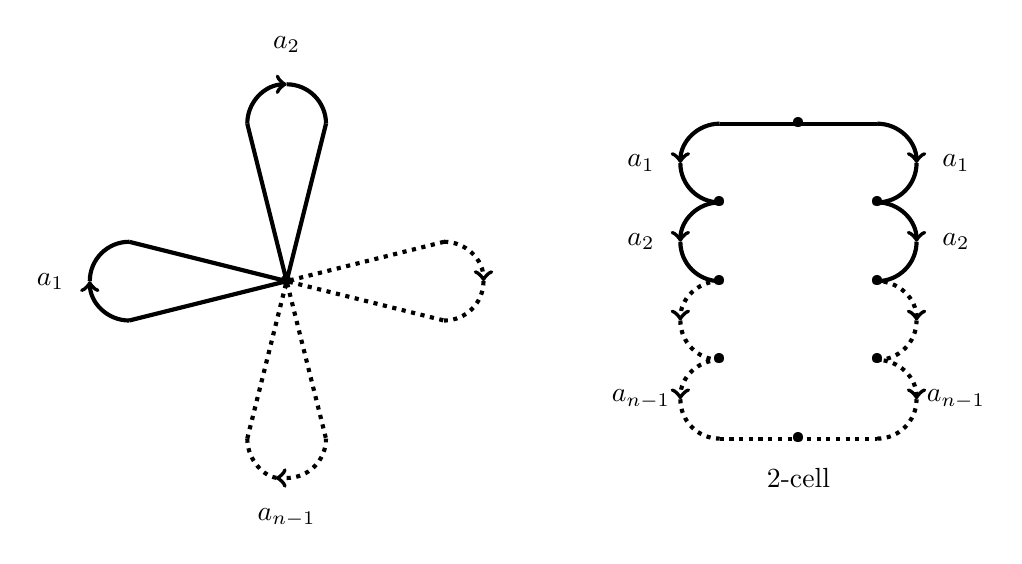
\begin{tikzpicture}
              %\draw[help lines](0,0) grid (12,6);
              \foreach\Point in {
                (3,3),
                (9.5,1), (9.5,5),
                (8.5,2), (8.5,3), (8.5,4),
                (10.5,2), (10.5,3), (10.5,4)
                }{\node at \Point {\textbullet};}
              \path[draw,dotted,line width=1.5pt] (8.5,1)--(10.5,1);
              \path[draw,line width=1.5pt] (8.5,5)--(10.5,5);
              \draw[line width=1.5pt,dotted] (10.5,1) arc (-90:0:0.5);
              \draw[line width=1.5pt,dotted] (10.5,2) arc (-90:0:0.5);
              \draw[line width=1.5pt] (10.5,3) arc (-90:0:0.5);
              \draw[line width=1.5pt] (10.5,4) arc (-90:0:0.5);

              \draw[line width=1.5pt,dotted,<-] (11,1.5) arc (0:90:0.5);
              \draw[line width=1.5pt,dotted,<-] (11,2.5) arc (0:90:0.5);
              \draw[line width=1.5pt,<-] (11,3.5) arc (0:90:0.5);
              \draw[line width=1.5pt,<-] (11,4.5) arc (0:90:0.5);

              \draw[line width=1.5pt,dotted,->] ( 8.5,2) arc (90:180:0.5);
              \draw[line width=1.5pt,dotted,->] ( 8.5,3) arc (90:180:0.5);
              \draw[line width=1.5pt,->] ( 8.5,4) arc (90:180:0.5);
              \draw[line width=1.5pt,->] ( 8.5,5) arc (90:180:0.5);

              \draw[line width=1.5pt,dotted] (8,1.5) arc (180:270:0.5);
              \draw[line width=1.5pt,dotted] (8,2.5) arc (180:270:0.5);
              \draw[line width=1.5pt] (8,3.5) arc (180:270:0.5);
              \draw[line width=1.5pt] (8,4.5) arc (180:270:0.5);

              \node[] at (11.5,1.5) {$a_{n-1}$};
              \node[] at (11.5,3.5) {$a_2$};
              \node[] at (11.5,4.5) {$a_1$};

              \node[] at (7.5,1.5) {$a_{n-1}$};
              \node[] at (7.5,3.5) {$a_2$};
              \node[] at (7.5,4.5) {$a_1$};
              \node[] at (9.5,0.5) {2-cell};

              \path[draw,line width=1.5pt,dotted] (2.5,1)--(3,3)--(3.5,1);
              \path[draw,line width=1.5pt] (2.5,5)--(3,3)--(3.5,5);
              \path[draw,line width=1.5pt,dotted] (5,3.5)--(3,3)--(5,2.5);
              \path[draw,line width=1.5pt] (1,3.5)--(3,3)--(1,2.5);

              \draw[line width=1.5pt,->] (2.5,5) arc (180:90:0.5);
              \draw[line width=1.5pt] (3,5.5) arc (90:0:0.5);
              \draw[line width=1.5pt,-<,dotted] (2.5,1) arc (-180:-90:0.5);
              \draw[line width=1.5pt,dotted] (3,0.5) arc (-90:0:0.5);
              \draw[line width=1.5pt,->,dotted] (5,3.5) arc (90:0:0.5);
              \draw[line width=1.5pt,dotted] (5.5,3) arc (0:-90:0.5);
              \draw[line width=1.5pt,->] (1,2.5) arc (-90:-180:0.5);
              \draw[line width=1.5pt] (0.5,3) arc (180:90:0.5);

              \node[] at (0,3) {$a_{1}$};
              \node[] at (3,6) {$a_{2}$};
              \node[] at (3,0) {$a_{n-1}$};
            \end{tikzpicture}
          \end{center}
        \end{proof}
    \end{enumerate}

  \item Carefully prove that the following are covering spaces.
    \begin{enumerate}
      \item
        \begin{enumerate}
          \item The map $\pi:\mathbb{C}\rightarrow\mathbb{C}^*$ defined by
            $\pi(z)=e^z$. \label{qn:exp}

            \begin{proof}
              First, we observe that the function is holomorphic, and hence
              is open and continuous by the open mapping theorem. Also,
              given any $y\in\mathbb{C}^*$, the inverse $z=\ln(y)$ always
              exists, and $\pi(z_1)=\pi(z_2)\leftrightarrow z_1-z_2\in
              2\pi\mathbb{Z}$. Hence, the map when restricted to any open
              subset of $\mathbb{R}\times[z-\pi i,z+\pi
              i)\subset\mathbb{C}^*$, where $z\in\mathbb{C}$, will be a
              homeomorphism when the codomain is the image of the subset.
              We use these properties to show that given any
              $y\in\mathbb{C}^*$, there is an open set $\mathcal{O}$
              containing $y$ such that its pre-image is composed of
              disjoint open sets each of which is homeomorphic to
              $\mathcal{O}$. \\

              Given $y\in\mathbb{C}^*$, choose any $z\in\mathbb{C}$ in
              its pre-image, and let $\mathcal{U}\in\mathbb{C}$ be an open
              ball $B_r(z)$ of radius $0<r<0.5$ around $z$. Let $\mathcal{O}$
              be the the image of $\mathcal{U}$ under $\pi$; this image
              will contain $y$ and is open because $\pi$ is an open
              function. Consider the restriction of $\pi$ to the open ball
              $\mathcal{O}$. Since the diameter of $\mathcal{O}$ is less
              than 1, the map is injective. Hence, by the holomorphic
              property of $\pi$, $\mathcal{U}$ is homeomorphic to
              $\mathcal{O}$. Now the pre-image of $\mathcal{O}$ is the
              union of $2\pi ki$ translations of $\mathcal{U}$ for
              $k\in\mathbb{Z}$, or more precisely
              
              \begin{equation*}
                \pi^{-1}(\mathcal{O}) = \bigcup\limits_{k\in\mathbb{Z}}
                (\mathcal{U}+2k\pi i),
              \end{equation*}

              where each $\mathcal{U}+2\pi ki=\{x+2k\pi
              i:x\in\mathcal{U}\}$ is open and homeomorphic to
              $\mathcal{O}$, which completes the proof. 
            \end{proof}

          \item For $n\in\mathbb{Z}\setminus\{0\}$, the map
            $\pi:\mathbb{C}^*\rightarrow\mathbb{C}^*$ defined by
            $\pi(z)=z^n$.

            \begin{proof}
              Similar to the proof in question~\ref{qn:exp}, observe that
              the map is holomorphic and is therefore open and continuous
              by the open mapping theorem. Also,
              given any $y\in\mathbb{C}^*$, the inverse $z=\ln(y)$ always
              exists, and $\pi(z_1)=\pi(z_2)\leftrightarrow z_1-z_2\in
              2\pi\mathbb{Z}$. Hence, the map when restricted to any open
              subset of $\mathbb{R}\times[z-\pi i,z+\pi
              i)\subset\mathbb{C}^*$, where $z\in\mathbb{C}$, will be a
              homeomorphism when the codomain is the image of the subset.
              We use these properties to show that given any
              $y\in\mathbb{C}^*$, there is an open set $\mathcal{O}$
              containing $y$ such that its pre-image is composed of
              disjoint open sets each of which is homeomorphic to
              $\mathcal{O}$. \\

            \end{proof}
        \end{enumerate}

      \item Prove that the map $\pi:\mathbb{C}\rightarrow\mathbb{C}$
        defined by $\pi(z)=z^2$ is not a covering space.
    \end{enumerate}
\end{enumerate}
\end{document}
